\documentclass[letterpaper,10pt,titlepage]{article}

\usepackage{graphicx}                                        
\usepackage{amssymb}                                         
\usepackage{amsmath}                                         
\usepackage{amsthm}                                          

\usepackage{alltt}                                           
\usepackage{float}
\usepackage{color}
\usepackage{url}

\usepackage{balance}
\usepackage[TABBOTCAP, tight]{subfigure}
\usepackage{enumitem}
\usepackage{pstricks, pst-node}

\usepackage{geometry}
\geometry{textheight=8.5in, textwidth=6in}

%random comment

\newcommand{\cred}[1]{{\color{red}#1}}
\newcommand{\cblue}[1]{{\color{blue}#1}}

\usepackage{hyperref}
\usepackage{geometry}

\hypersetup{
  colorlinks = true,
  urlcolor = black,
  pdfauthor = {\name},
  pdfkeywords = { CS434 ``Machine Learning'' },
  pdftitle = { Linear Regression and the Perceptron},
  pdfsubject = { CS434},
  pdfpagemode = UseNone
}

\begin{document}
\begin{flushright}
\end{flushright}
\begin{flushleft}
\textbf Eric Zounes, Ian Fridge \\
\today  \\
CS434: Assignment 1 
\end{flushleft}
\section[1]{Implementation Assignment} 
\large Plots for problems 1, 2, and 3. \\ 

The accuracy for unshuffled test data at epoch 20 to 100 by steps of 20: Unreliable because of the first data point. Decision boundary is heavily skewed. The accuracy for shuffled test data  at epoch 20 to 100 by steps of 20 is: 97/99, 97/99, 98/99, 1, 1. This shows that our algorithm is much more effective when the data points are randomly chosen. \\
Accuracy for unshuffled training data at epoch 20 to 100 by steps of 20: 98/99, 91/99, 1, 1, 1. The perceptron seems to make a large amount of error at 40 epochs. Overfitting could contribute to misclassification at certain points between 20 and 60 epochs. For shuffled training data at epoch 20 to 100 by steps of 20: 92/98, 1, 1, 1, 1. There is a large amount of error at 20 epochs but we can see that it quickly converges. 
\begin{figure}[th!]
\centering
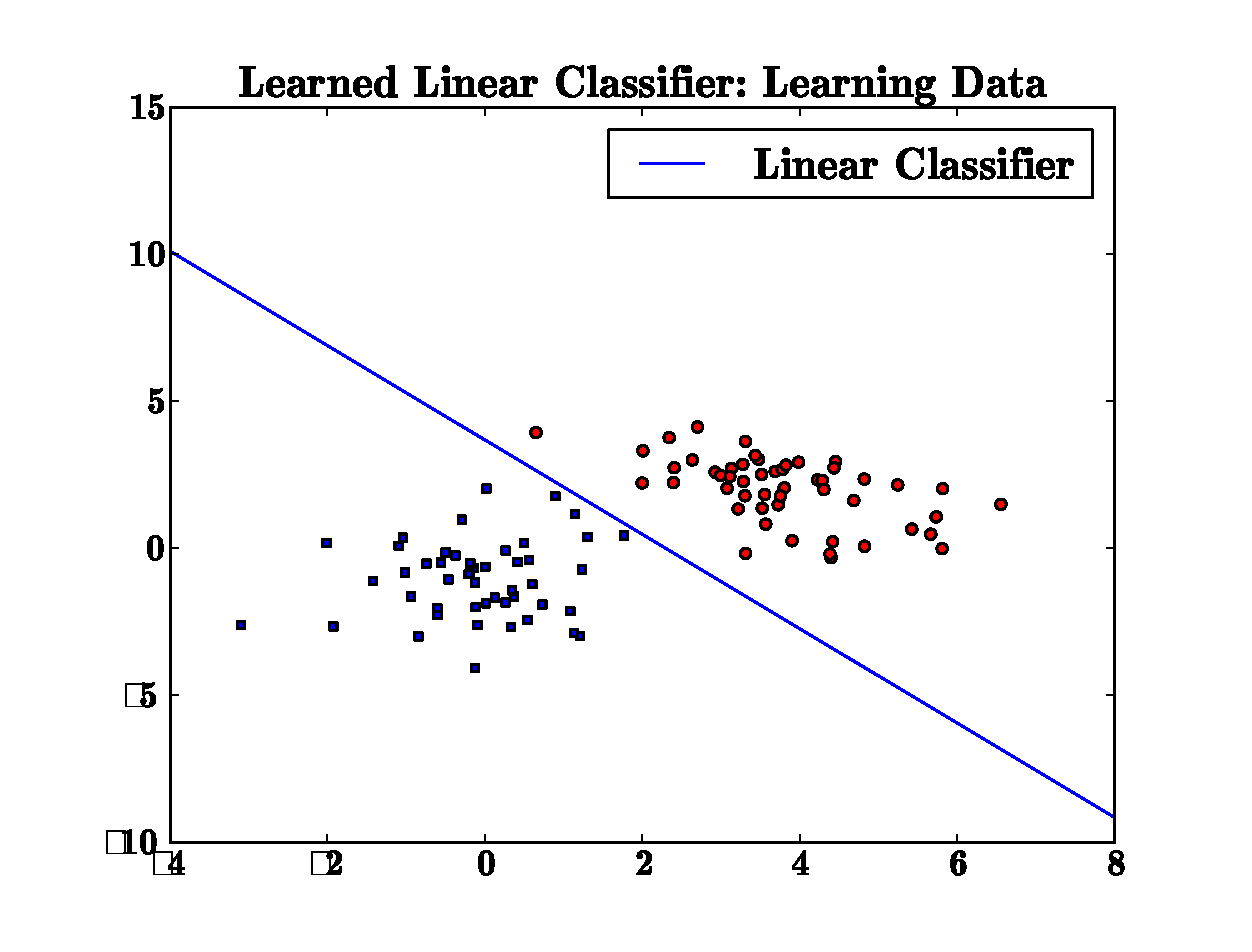
\includegraphics[width=5in]{learn.eps} 
\end{figure} 
\\[5mm]
\begin{figure}[th!]
\centering
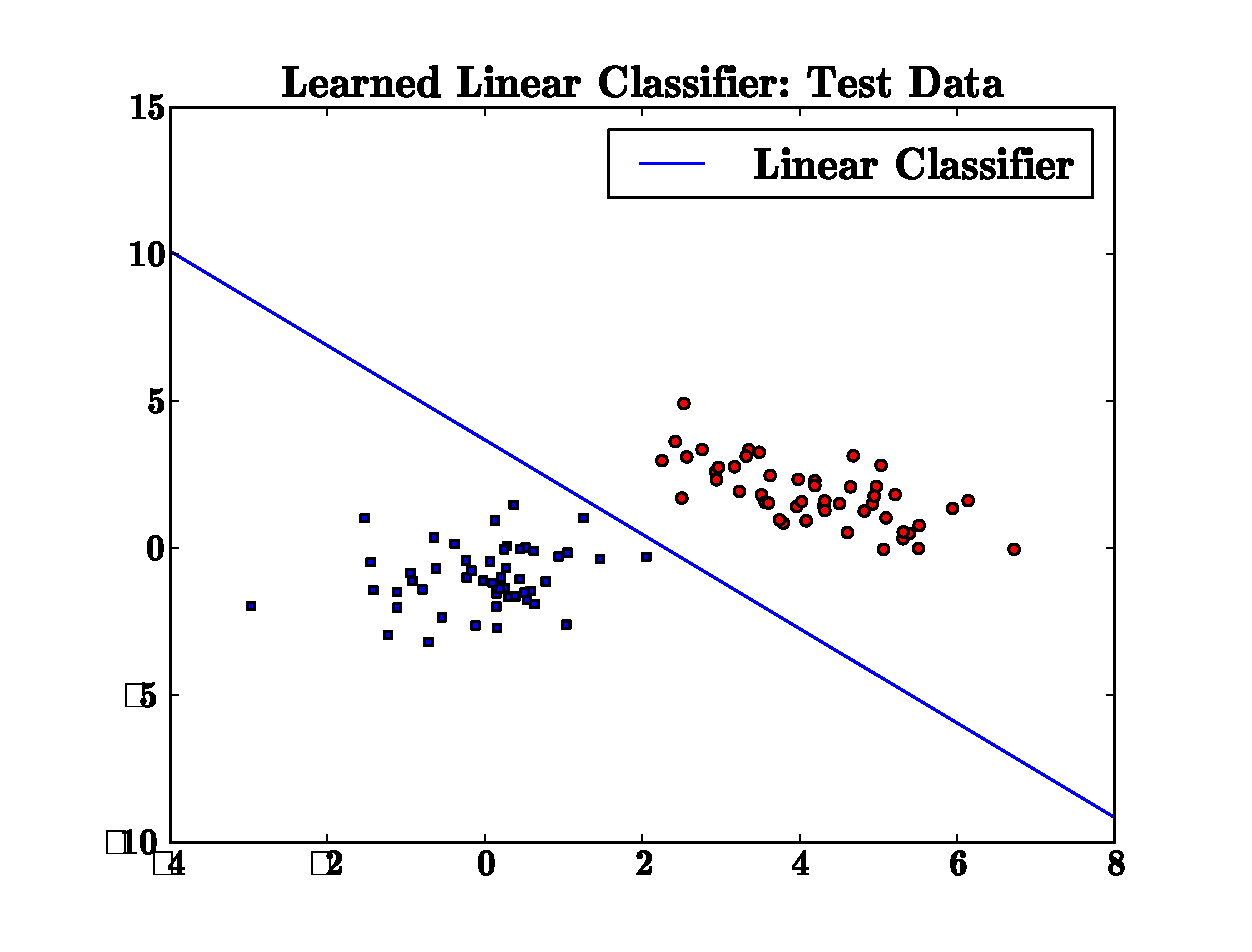
\includegraphics[width=5in]{test.eps} 
\end{figure} 
\\[5mm] 
\pagebreak
\begin{figure}[th!]
\centering
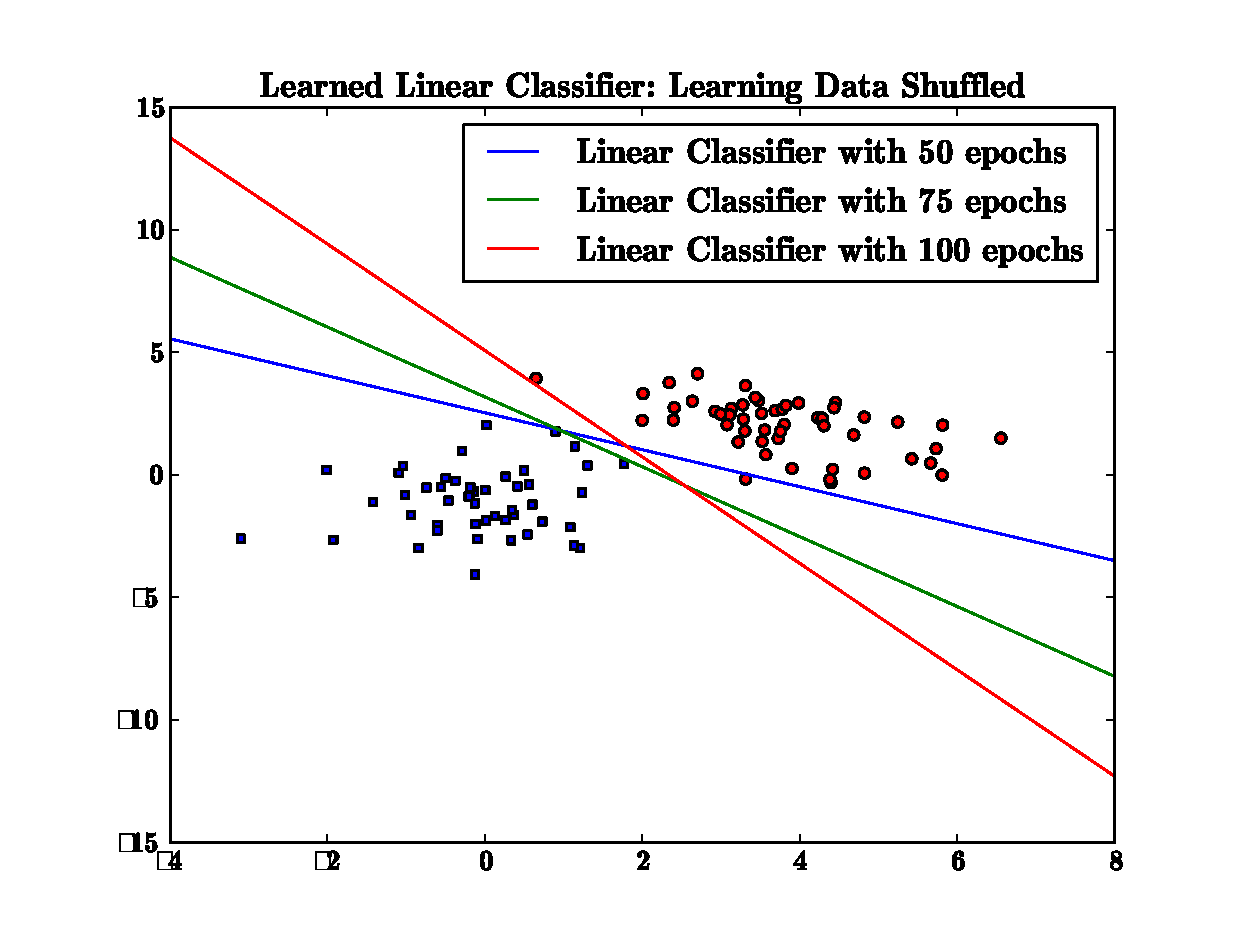
\includegraphics[width=5in]{shuffled.eps} 
\end{figure} 
\\[5mm] 
\begin{figure}[th!]
\centering
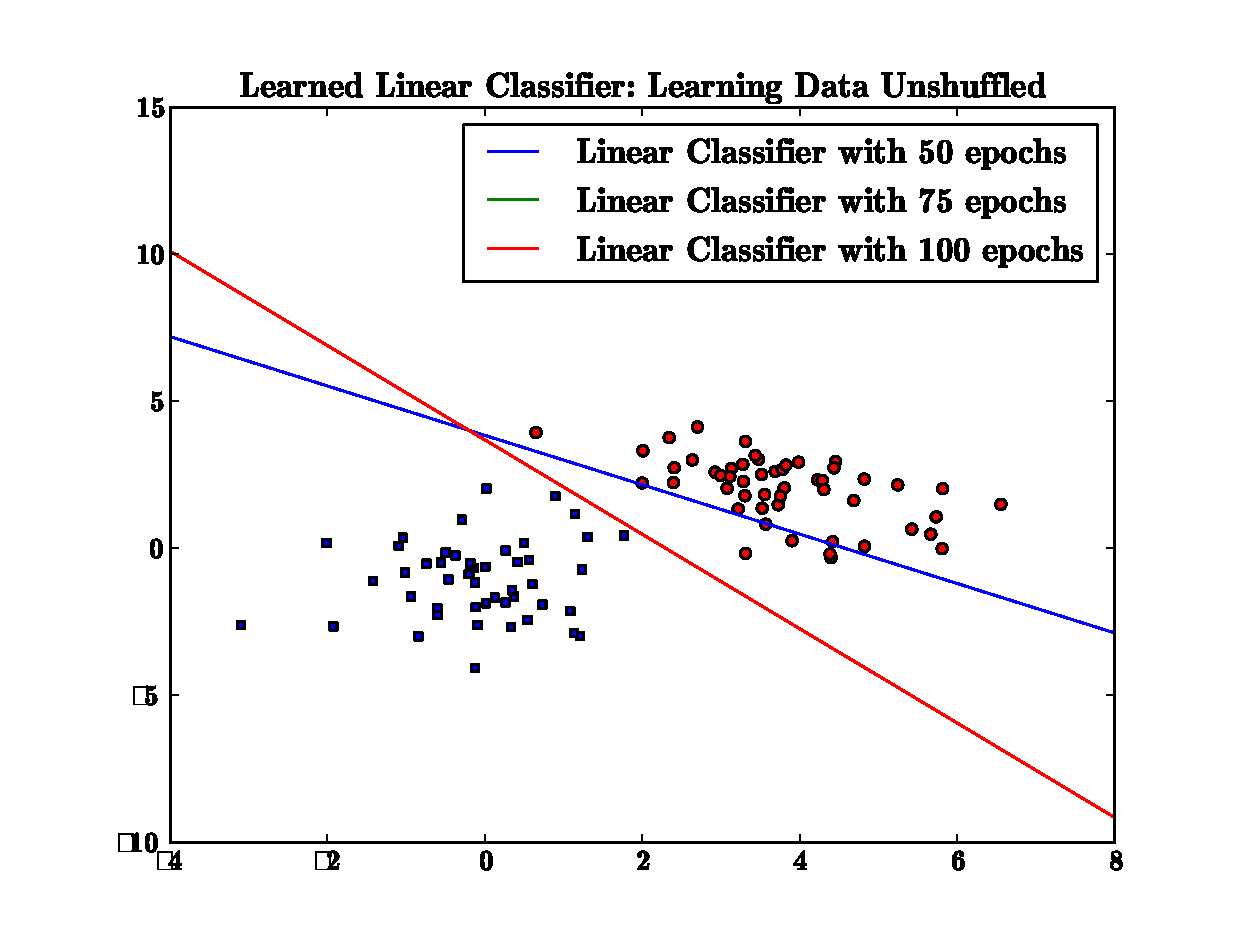
\includegraphics[width=5in]{unshuffled.eps} 
\end{figure} 
\\[5mm]
\pagebreak
\begin{figure}[th!]
\centering
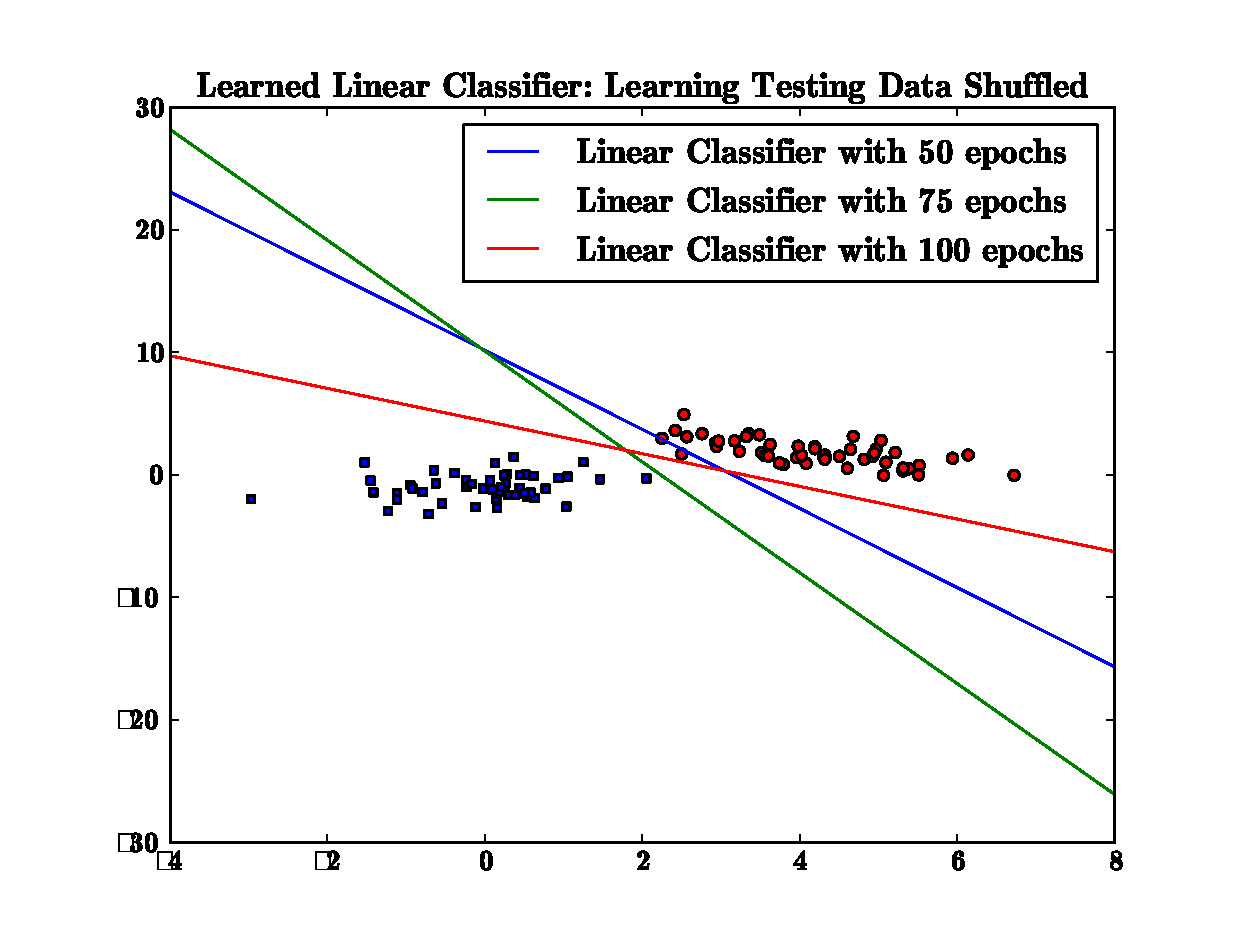
\includegraphics[width=5in]{test_data_shuffled.eps} 
\end{figure} 
\pagebreak
\pagebreak
\begin{figure}[th!]
\centering
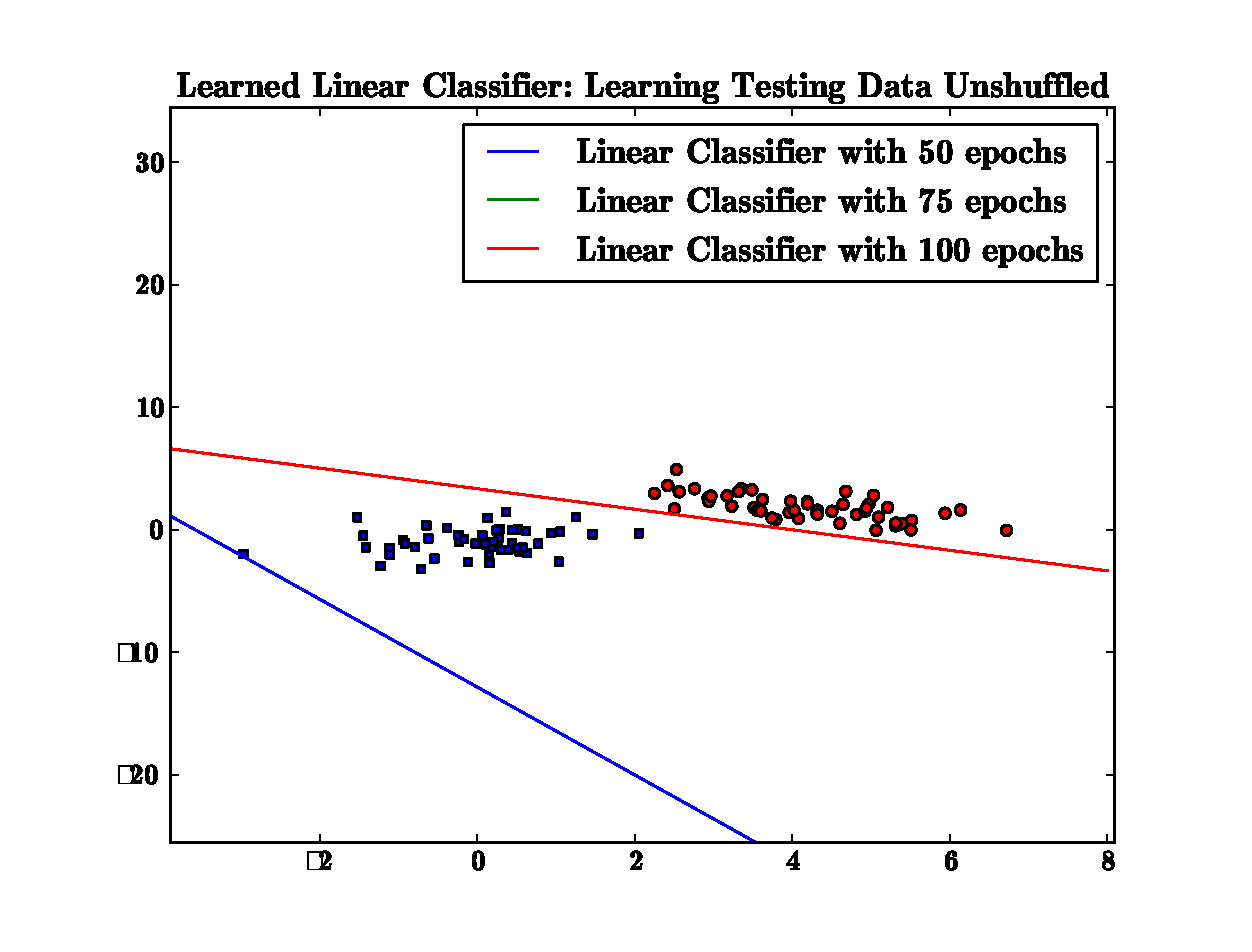
\includegraphics[width=5in]{test_data_unshuffled.eps} 
\end{figure} 
\pagebreak
\\[15mm]
\section[2]{Individual Assignment} 
\begin{enumerate} 
	\item Design your supervised learning problem. In this class, we will spend one class discussion a particular learning task and try to come up with a machine learning solution to the problem. I would like everyone in the class to contribute a candidate task for this case study. In particular, please provide one supervised learning tasks that you think is cool and interesting. Describe the task, explain why you think this is (or can be solved as) a supervised learning task (what is the target variable that you want to predict, and what are the input features you might use). Whoever proposes the task that is chosen for the case study will get 10 bonus points. \\

 Supervised learning algorithms are well suited for problems where there are consistent patterns influenced by one or more independent variables. The algorithms which can solve these problems are relatively easy to understand in that they predict a rate of change given a set of training data. Learning algorithms are most effective when operating on data which is linearly separable. So, it is important that there are definite correlations in our training data. A great application of supervised learning is predicting traffic density based on weather forecast. In order to design an effective solution for this problem we'll first start sampling our training data at uniform intervals. We must agree on quantifiable features which, we suspect, have an effect on our dependent variable. For example, our features could consist of temperature, wind speed, and cloud coverage. These are all valid features which have potential to affect traffic density. To measure the effect we'll also define a threshhold for the traffic density in order to create a classifier. Thus, we have average traffic density act as a linear classifier. A decision tree algorithm would work well for this type of problem due to the relationship between features. For example, there might be an obvious trend in temperature vs. cloud coverage. \\[15mm]

	\item Below is the set of training data that was used in class for linear regression. Please complete the following tasks using this data.

	\begin{enumerate} 	
		\item  Using only knee height we find that b $=82.87$ and w1 $= 1.81$ SSE $= 25.879$. \\

\begin{figure}[th!]
\centering
\includegraphics[width=5in]{Kneeheight_training.eps} 
\end{figure} 
\\[10mm]
		\item Using both of the independent variables we find that the value of b $= 71.315$ and w1 $= .79$, w2 $= .323$ \\
SSE for the arm span is $= 15.93$ \\
\\[5mm]
\begin{tabular}{ | c | c | c | c | c | p{10cm} | }
\hline
Knee Height & Arm Span & Projected & Actual & Error \\ \hline
50.000      & 166.000  & 171.855   & 170.000 & 1.855 \\
57.000      & 196.000  & 187.693   & 191.000 & 3.307 \\
50.000      & 191.000  & 180.442   & 189.000 & 8.558 \\
53.340      & 180.340  & 179.421   & 180.340 & 0.919 \\
54.000      & 174.000  & 177.765   & 171.000 & 6.765 \\
55.880      & 176.530  & 180.120   & 176.530 & 3.590 \\
57.000      & 177.000  & 181.167   & 187.000 & 5.833 \\
55.880      & 208.280  & 191.025   & 185.420 & 5.605 \\
57.000      & 199.000  & 188.723   & 190.000 & 1.277 \\
54.000      & 181.000  & 180.169   & 181.000 & 0.831 \\
55.000      & 178.000  & 179.930   & 180.000 & 0.070 \\
53.000      & 172.000  & 176.288   & 175.000 & 1.288 \\
55.880      & 208.280  & 191.025   & 185.420 & 5.605 \\
57.000      & 199.000  & 188.723   & 190.000 & 1.277 \\
54.000      & 181.000  & 180.169   & 181.000 & 0.831 \\
55.000      & 178.000  & 179.930   & 180.000 & 0.070 \\
53.000      & 172.000  & 176.288   & 175.000 & 1.288 \\
57.000      & 185.000  & 183.915   & 188.000 & 4.085 \\
49.500      & 165.000  & 171.117   & 170.000 & 1.117 \\
57.000      & 188.000  & 184.945   & 185.000 & 0.055 \\ \hline
\end{tabular} 
\\[10mm]
		\item The SSE was greater for knee height because of an outlier. Weight might reduce the amount of error gained from the knee height feature as it is less reliable than arm span. \\
	\end{enumerate} 
	\item Below is a set of 2-d data points, with black dots representing positive class and red dots representing negative class. The blue line segments show the Voroni diagram of these points.  \\
	\begin{enumerate}
		\item  What are the training error and leave-one-out error of 1-nearest neightbor? \\
			Training error for:  1-nearest neighbor $= 0$ \\
	   	        Leave-one-out error for: 1-nearest neighbor $= 6$ \\
		\item  What are the training error and leave-one-out error of 3-nearest neighbor? \\
	  	        Training error for:  3-nearest neighbor $= 2$ \\ 
	                Leave-one-out error for: 3-nearest neighbor $6$ \\
		\item  Decision boundary for 1-nearest neighbor \\[5mm]

\begin{figure}[th!]
\centering
\includegraphics[width=5in]{1-neighbor-decision.eps} 
\end{figure} 
 
\\[5mm]

d. I'm assuming the question is asking if the answer will differ from "c" because "a" did not return a subset of lines. The answer is false because the data can't be correctly partitioned  	by drawing a different decision boundary. 


\end{document}
